% This is samplepaper.tex, a sample chapter demonstrating the
% LLNCS macro package for Springer Computer Science proceedings;
% Version 2.20 of 2017/10/04
%
\documentclass[runningheads]{llncs}
%
\usepackage{graphicx}
\usepackage{amsmath}
% Used for displaying a sample figure. If possible, figure files should
% be included in EPS format.
%
% If you use the hyperref package, please uncomment the following line
% to display URLs in blue roman font according to Springer's eBook style:
% \renewcommand\UrlFont{\color{blue}\rmfamily}

\begin{document}
%
\title{Aggregated Financial Forecasting Calculation in Human-Computer Distributed Computing\thanks{This research is funded by Velbazhd Software LLC and it is partially supported by the Bulgarian Ministry of Education and Science (contract D01–205/23.11.2018) under the National Scientific Program ``Information and Communication Technologies for a Single Digital Market in Science, Education and Security (ICTinSES)'', approved by DCM \# 577/17.08.2018.}}
%
\titlerunning{Aggregated FF Calculation in HCDC}
% If the paper title is too long for the running head, you can set
% an abbreviated paper title here
%
\author{Petar Tomov \and Iliyan Zankinski \and Todor Balabanov\orcidID{0000-0003-3139-069X}}
%
\authorrunning{P. Tomov et al.}
% First names are abbreviated in the running head.
% If there are more than two authors, 'et al.' is used.
%
\institute{Institute of Information and Communication Technologies \\ Bulgarian Academy of Sciences \\ acad. Georgi Bonchev Str., block 2, 1113 Sofia, Bulgaria \\ \email{p.tomov@iit.bas.bg} \email{iliyan@hsi.iccs.bas.bg} \email{todorb@iinf.bas.bg}
\url{http://iict.bas.bg/}}
%
\maketitle              % typeset the header of the contribution
%
\begin{abstract}
Three of the most famous financial forecasting donated distributed computing projects for the last decade were MoneyBee, GStock and MQL5 Cloud Network. The idea of a desktop computer screen-saver used for artificial neural networks training was extended in VitoshaTrade project where Android Active Wallpaper is used for the same purpose. The project implementation goes on in IICT-BAS and the forecasting capabilities are evolved in the direction of human-computer based distributed computing. This research proposes financial forecasting calculation based on users' classification and votes given for the particular financial future events. 

\keywords{Financial forecasting \and Distributed computing \and Voting platform.}
\end{abstract}
%
%
%
\section{Introduction}
%
Three of the most famous financial forecasting donated distributed computing projects for the last decade were MoneyBee \cite{money-bee-01}, GStock \cite{g-stock-01} and MQL5 Cloud Network \cite{mql5-cloud-network-01}. MoneyBee project was organized as donated distributed computing screen-saver. Artificial neural networks were trained to forecast financial time series during desktop computers idle usage. GStock project used donated distributed computing for trading strategies testing. Many different investment strategies were checked over historical data and the best suited were applied for buy/sell signals generation. MQL5 Cloud Network is paid distributed computing platform in which trading strategies can be tested. 

The idea of a desktop computer screen-saver used for artificial neural networks training was extended in VitoshaTrade \cite{vitosha-trade-01} project where Android Active Wallpaper is used for the same purpose. The project implementation goes on in IICT-BAS and the forecasting capabilities are evolved in the direction of human-computer based distributed computing (crowdsensing \cite{crowdsensing-01}). The users are asked to vote \cite{voting-01} for the future change in the price of Forex currency pairs. Android operating system provides the ideal user interface capabilities for such voting by its widget components. By HTTP protocol the vote of the users is collected on a remote PHP-MySQL based server. As proposed in NSFDE\&A'20, users' votes are classified in four categories: 1) High voting frequency and high guess rate users; 2) Low voting frequency and high guess rate users; 3) High voting frequency and low guess rate users; 4) Low voting frequency and low guess rate users.

This research proposes financial forecasting calculation based on users classification and votes given for particular financial future event. The rest of this paper is organized as follows: Section 1 describes the problems related to financial forecasting and states the ideas for computing in a distributed environment; Section 2 proposes a practical solution for a mobile distributed voting solution; Section 3 reveals some practical experiments and related results; and Section 4 concludes with some suggestions for further work.
%
\subsection{Financial Time Series}
%
Time series are values measured in strict time order \cite{time-series-01}. In most of the cases, measurements are done in equal time intervals, but exceptions also do exist \cite{time-series-02}. The result of such measurements is discrete time-ordered data. There are many natural processes that can be described with time series as average daily temperature, count of sunspots number of flu sick people, values of the prices and many others \cite{time-series-03}. Time series are useful in almost every domain where measurements can be done in temporal order. Line charts are the most used tool for visualization of time series. 

Technical analysis of financial time series uses a group of methods for temporal data analyzing in such a way that meaningful statistics and other characteristics to be extracted. Financial time series forecasting is based on a model that predicts future values according to previously observed values. Financial time series usually have trend, seasonality and high-frequency oscillations \cite{time-series-04}. The base of the technical analysis in financial time series is an appropriate curve fitting to the points which are already known.
%
\subsection{Distributed Computing in Financial Forecasting}
%
When a particular computation is a too much time consuming it is rational such calculation to be done on many computational machines in parallel \cite{distributed-computing-01}. When artificial neural networks are used for financial time series forecasting, the training can be organized with genetic algorithms \cite{genetic-algorithms-01} or differential evolution \cite{differential-evolution-01}. Both global optimization techniques are perfect for parallel computing and of course for distributed computing because global population can be separated in many local populations and the process of optimization can go simultaneously.
%
\begin{figure}
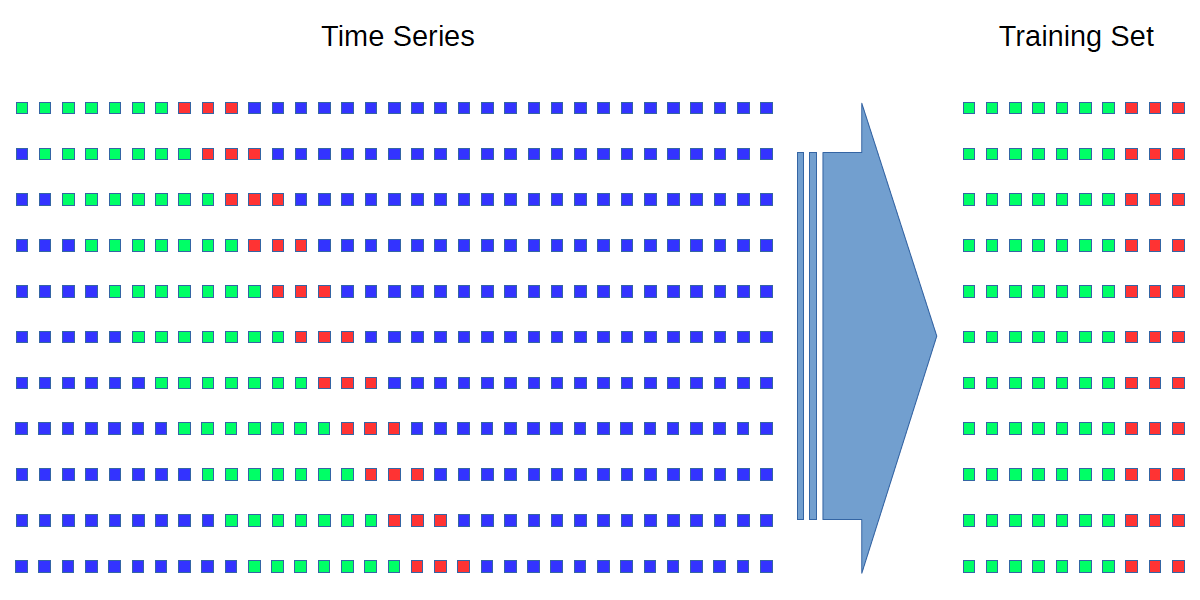
\includegraphics[width=\textwidth]{fig01.png}
\caption{Time series splitting to training examples.}
\label{fig01}
\end{figure}
%
\begin{figure}
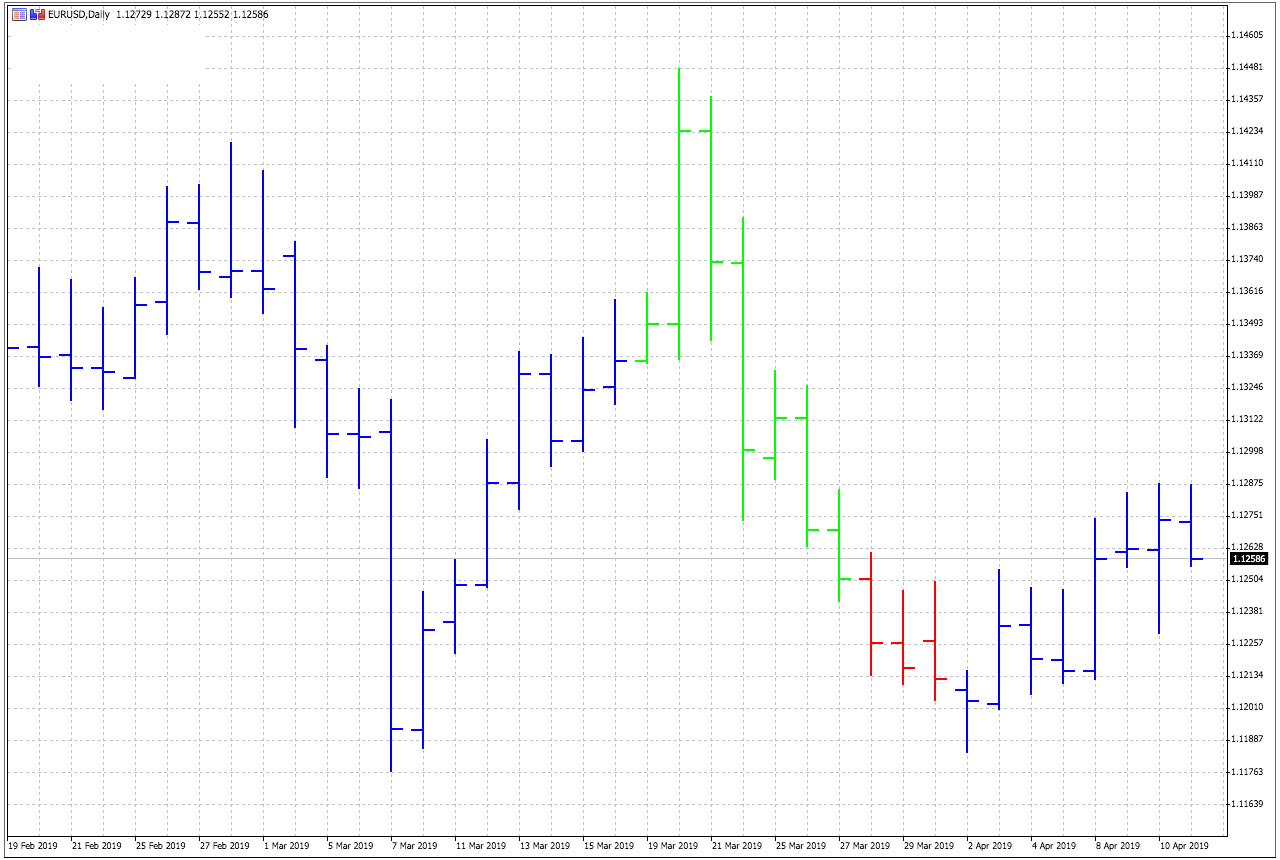
\includegraphics[width=\textwidth]{fig02.png}
\caption{Financial time series.}
\label{fig02}
\end{figure}
%
In the technical analysis time series are conditionally divided (Fig. \ref{fig01} and Fig.\ref{fig02}) into past (lag) and future (lead) periods \cite{time-series-04}. Training examples are loaded as input in the artificial neural network \cite{time-series-04} and the prediction is expected on the output (Fig. \ref{fig03}). The training process on the local devices goes into two common phases, which are related to the way the population individual are represented. Artificial neural network topology is predefined and its optimization is beyond the scope of this approach, but the weights of the artificial neural network are subject to optimization. The population of the evolutionary algorithm is organized as sets of artificial neural networks weights matrices. Each set of weights (population individual) is provided to the back-propagation training procedure until there is no significant improvement of the forecasting capabilities. After that crossover and mutation are applied and a new generation is added to the population. Uniform crossover is used as the best way to prevent total information destruction in an artificial neural network. Newly created individuals are also trained with back-propagation algorithm and the evolution algorithm goes continuously. 
%
\begin{figure}
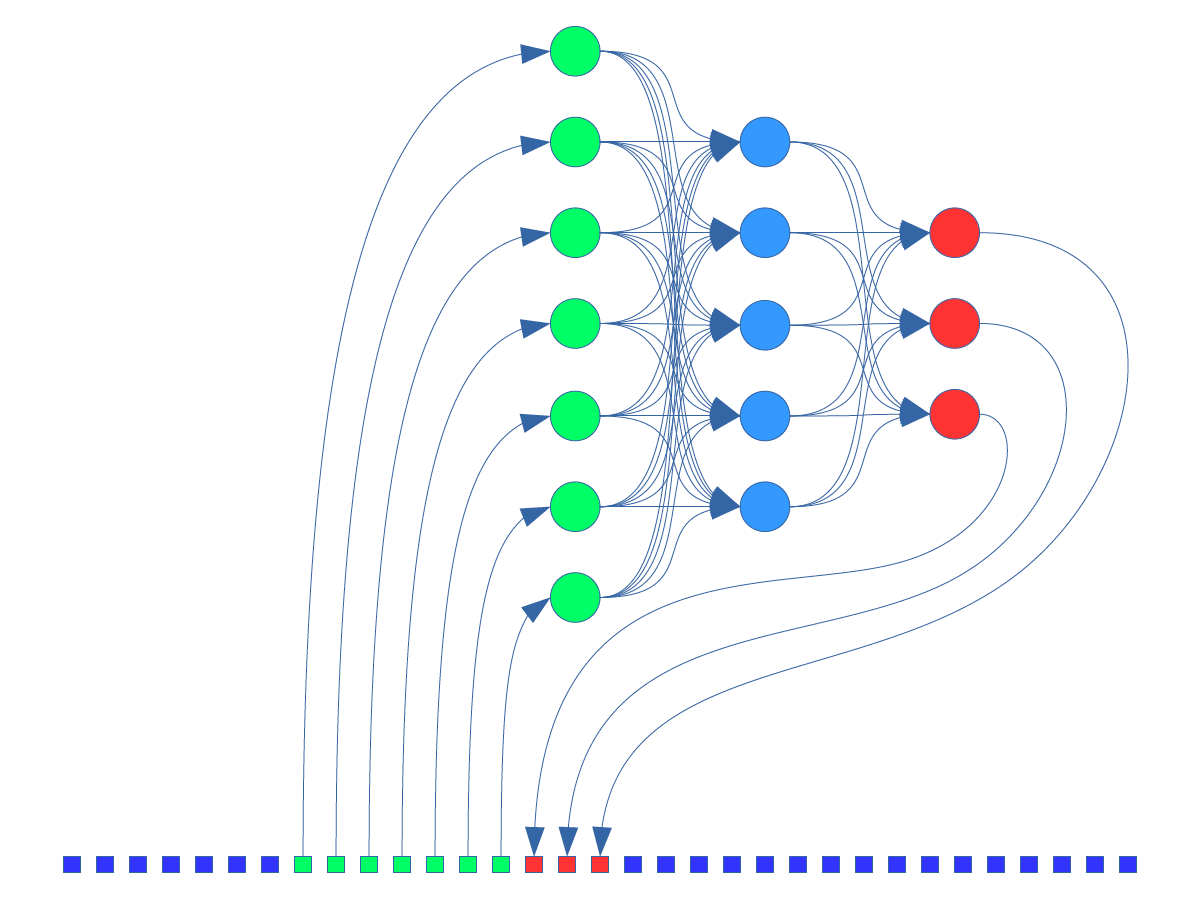
\includegraphics[width=\textwidth]{fig03.png}
\caption{Artificial neural network training.}
\label{fig03}
\end{figure}
%
Such symbolic restarting of the back-propagation training has wide similarity with simulated annealing. After the crossover and the mutation operators weights of the artificial neural network are partially distressed and disordered. This helps the back-propagation training to proceed from a previous point of the training process and to escape possible local optimums. When this hybrid training is done on mobile devices the training process goes 24/7. The best-found weights of an artificial neural network are reported to the remote server. In this way, best-found individuals form a global evolutionary algorithm population. 
%
\section{Android OS Crowdsensing Solution}
%
Distributed computing forecasting described in the previous section is very attractive and very cost-efficient, but it has a common disadvantage - subjective human opinion is not taken in any form. It is very well known that financial markets are extremely volatile. Global disasters like the COVID-19 pandemic are capable to put financial markets in a highly-unpredictable state. In such extreme situations, pure technical analysis is useless. 
%
\begin{figure}
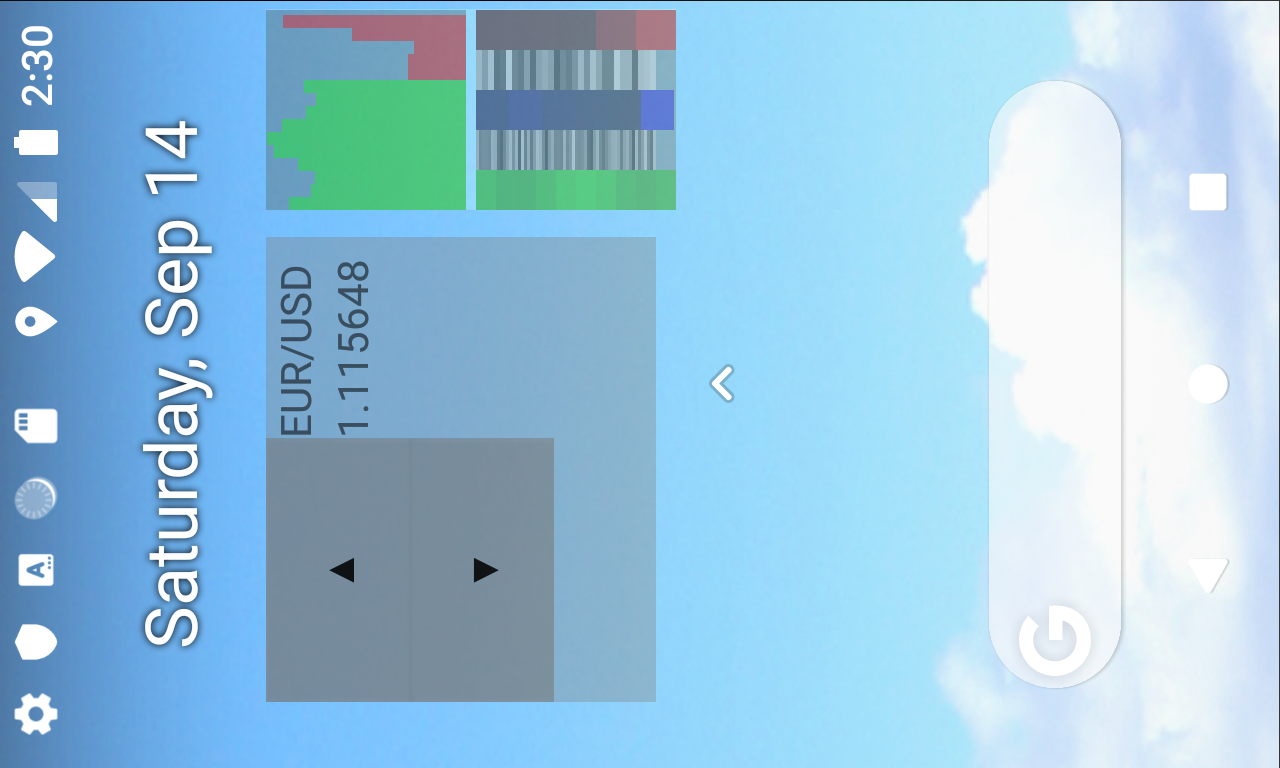
\includegraphics[width=\textwidth]{fig04.png}
\caption{Android OS voting interface.}
\label{fig04}
\end{figure}
%
Subjective human opinion in the shape of human intuition can improve forecasting results significantly in situations where methods of pure applied mathematics are not applicable. Human intuition is not completely understood yet, but it is based on rich life experiences and subconscious information processing in the human brain. This research purposes aggregation of the information collected from a mobile device voting system (Fig. \ref{fig04}) and forecasting improvement with the aggregated data in use.

Users have the opportunity to vote for future changes in the particular financial time series. The vote is collected on a remote server. Voters are classified in four common groups: High voting frequency and high guess rate users (group $a$); Low voting frequency and high guess rate users (group $b$); High voting frequency and low guess rate users (group $c$); Low voting frequency and low guess rate users (group $d$). This classification is the base of the aggregated forecasting proposed in this research. Each group of the voters participates with a different coefficient in the final forecast calculation. 
%
\begin{equation}
\begin{array}{l}
f(x) = \frac{w_{a}}{n_{a}} \sum_{a=1}^{n_{a}} x_{a} + \frac{w_{b}}{n_{b}} \sum_{b=1}^{n_{b}} x_{b} + \frac{w_{c}}{n_{c}} \sum_{c=1}^{n_{c}} x_{c} + \frac{w_{d}}{n_{d}} \sum_{d=1}^{n_{d}} x_{d} \\
\text{where} \\
N = n_{a} + n_{b} + n_{c} + n_{d} \\
w_{a} + w_{b} + w_{c} + w_{d} = 1
\end{array}
\label{equ01}
\end{equation}
%
When a particular forecast should be issued single votes for the particular situation are taken and they are aggregate by groups to form the forecast. The forecast is in the form of chance the price to go up (value between 0.0 and 1.0, Eq. \ref{equ01}) and the opposite chance for the price to go down (also between 0.0 and 1.0). The sum of the two chances gives 1. The vector $x$ in Eq. \ref{equ01} is a binary vector. It has 1 for each vote of a user who thinks that the price will go up and it has 0 for each vote of the user who thinks that the price will go down. The total number of available votes for a particular forecasted event is $N$. The size of each group is given by the small letter $n$ with an index. Each group participate in the aggregated forecast with a given coefficient presented by the small letter $w$ with and index. The values of the coefficients are subject to a multicriteria problem and are chosen by the decision-makers.
%
\section{Experiments \& Results}
%
\section{Conclusions}
%
% ---- Bibliography ----
%
% BibTeX users should specify bibliography style 'splncs04'.
% References will then be sorted and formatted in the correct style.
%
% \bibliographystyle{splncs04}
% \bibliography{mybibliography}
%
\begin{thebibliography}{8}

\bibitem{money-bee-01} Bohn, A., Guting, T., Mansmann, T.: MoneyBee Aktienkursprognose mit kunstlicher intelligenz bei hoher rechenleistung. Wirtschaftsinf \textbf{45}, 325--333 (2003)

\bibitem{g-stock-01} Chokesatean, P.: Credibility-based Binary Feedback Model for Grid Resource Planning. University of Pittsburgh (2008)

\bibitem{mql5-cloud-network-01} Chang, C., Narayana Srirama S., Buyya, R.: Indie Fog An Efficient Fog-Computing Infrastructure for the Internet of Things. Computer \textbf{50}(9), 92--98 (2017)

\bibitem{vitosha-trade-01} Zankinski, I., Barova, M., Tomov P.: Hybrid Approach Based on Combination of Backpropagation and Evolutionary Algorithms for Artificial Neural Networks Training by Using Mobile Devices in Distributed Computing Environment. Proceedings of Large-Scale Scientific Computing, 425--432 (2018)

\bibitem{crowdsensing-01} Leppanen, T., Alvarez Lacasia, J., Tobe, Y., Sezaki, K., Riekki, J.: Mobile crowdsensing with mobile agents. Autonomous Agents and Multi-Agent Systems \textbf{31}, 1--35 (2017)

\bibitem{voting-01} Laukkanen, S., Kangas, A., Kangas, J.: Applying voting theory in natural resource management A case of multiple-criteria group decision support, Journal of Environmental Management, \textbf{64}(2), 127--137 (2002)

\bibitem{time-series-01} Bandt, C., Pompe, B.: Permutation Entropy A Natural Complexity Measure for Time Series. Physical Review Letters, \textbf{88}(17), 174102 (2002)

\bibitem{time-series-02} Salvador, S., Chan, P.: Toward Accurate Dynamic Time Warping in Linear Time and Space. Intelligent Data Analysis, \textbf{11}(5) 561--580 (2007)

\bibitem{time-series-03} Lan, Y.: Computational Approaches for Time Series Analysis and Prediction Data-Driven Methods for Pseudo-Periodical Sequences. University of Bradford (2009)

\bibitem{time-series-04} Kolev, K., Sevova, J., Ketipov, R., Blagoev, I., Petrov, P., Kostadinov, G., Zankinski, I.: Removal of Linear Component and Sinusoidal Harmonics from Time Series with Differential Evolution. Proceedings of Annual University Scientific Conference of Vasil Levski National Military University, 1586--1594 (2019)

\bibitem{distributed-computing-01} Megiddo, N.: Applying parallel computation algorithms in the design of serial algorithms. Journal of the Association for Computing Machinery \textbf{30}(4), 852--865 (1983)

\bibitem{genetic-algorithms-01} Donate, J.P., Li, X., Sanchez, G.G., Miguel, A.S.: Time series forecasting by evolving artificial neural networks with genetic algorithms, differential evolution and estimation of distribution algorithm. Neural Computing and Applications \textbf{22}, 11--20 (2013)

\bibitem{differential-evolution-01} Balabanov, T. Zankinski, I., Dobrinkova, N.: Time Series Prediction by Artificial Neural Networks and Differential Evolution in Distributed Environment. Proceedings of Large-Scale Scientific Computing Conference \textbf{7116}, 198--205 (2012)

\bibitem{time-series-04}  Tomov, P., Zankinski, I., Balabanov, T.: Training of Artificial Neural Networks for Financial Time Series Forecasting in Android Service and Widgets. Problems of Engineering Cybernetics and Robotics \textbf{71}, 50--56 (2019)

\end{thebibliography}

\end{document}
